% Drawing 136/18-2 -- folder 136, batch 18, archive page 358 (PDF page 359).
% Transcription: une petite sphère hachurée, cerclée d’un équateur épais.
% Kind: small hatched sphere with thick equator. Method 2 (schematic redraw from the facsimile). Status: ok.
% Notes: A small sphere, hatched, girdled by a thick equator.
% Coordinates: 1 unit = 1 mm = 1/100 of the crop width (bbox in page fractions: [0.21, 0.455, 0.27, 0.49]).
% Redrawn by Claude (claude-opus-5-5), issue #73, 2026-11-07; not checked by a human; not compiled (no TeX in the session).
% Rights: reproduces part of the work -- behind RENDER_TRANSCRIPTS, never published by itself.
\documentclass[tikz,border=3pt]{standalone}
\usepackage{amsmath,amssymb}
\usetikzlibrary{patterns,arrows.meta}
\tikzset{pencil/.style={black!45}, struck/.style={black!35}, mark/.style={circle,draw,inner sep=1.3pt}, pt/.style={circle,fill,inner sep=0.9pt}, opt/.style={circle,draw,fill=white,inner sep=1.1pt}}
\begin{document}
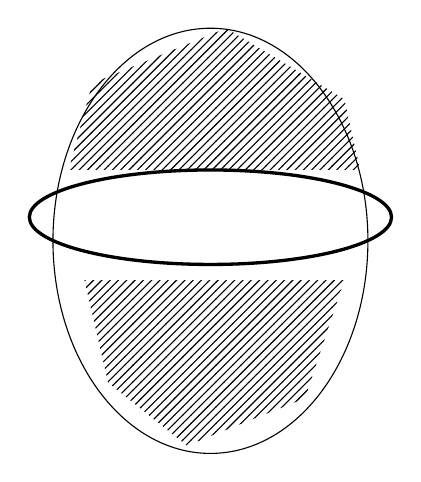
\begin{tikzpicture}[x=1mm,y=1mm,line cap=round,line join=round,font=\scriptsize]
\draw (43,-40) ellipse[x radius=20, y radius=27];
\draw[very thick] (43,-37) ellipse[x radius=23, y radius=6];
\fill[pattern=north east lines] (28,-20) -- (45,-13) -- (60,-22) -- (62,-31) -- (25,-31) -- cycle;
\fill[pattern=north east lines] (27,-45) -- (60,-45) -- (55,-60) -- (40,-66) -- (30,-58) -- cycle;
\end{tikzpicture}
\end{document}
